
\section{Average Linkage HAC on Paths in \NC}\label{sec:pathupperbound}
In this section, we present an $\tilde{O}(n)$ work and $O(\mathsf{polylog}(n))$ depth algorithm for solving average linkage HAC on path graphs, provided that the aspect ratio of the input instance is bounded by $\poly(n)$.
%\kgnote{discuss/define aspect ratio earlier} 
%\hnote{Better exclude weight-zero edges in defn}
The {\em aspect ratio} is defined as $\mathcal{A} = W_{\max}/W_{\min}$, where $W_{\max} = \argmax_{e \in E} w(e)$ and $W_{\min} = \argmin_{e\in E} w(e)$ (note that this definition excludes all non-edges, which implicitly have a weight of 0).
The main algorithm for this section is presented in Algorithm~\ref{alg:paths}, which we first give a high-level overview of next, followed by a detailed description.


\begin{algorithm}[ht]
\caption{Average linkage HAC on paths; $\mathtt{ProcessChain}$ assumes that the input chain has a certain structure. However, this assumption can be removed easily (see \Cref{sec:pathupperbound})}\label{alg:paths}
\SetKwInput{Input}{Input}
% \KwIn{A path graph $G = (V, E, w)$}
\SetKwFunction{FHac}{PathHAC}
\SetKwFunction{Fchain}{ProcessChain}
\SetKwProg{Fn}{Function}{:}{}
\SetKwProg{parfor}{parallel for}{:}{}

\Input{A path graph $G = (V, E, w)$}
\Fn{\FHac{$x, y, w, S$}}{
Compute buckets $B_1,B_2,\ldots,B_T$ such that $B_i$ contains edges with weights in $((2/3)^{t}w_{\max}, (2/3)^{t-1}w_{\max}]$.\\
\For{$t=1$ to $T$}{
Let $\mathcal{C} \gets$ Nearest-neighbor chains on the induced graph $G[B_t]$.\\
\parfor{each $C \in \mathcal{C}$}{
\Fchain{$C$}
}
}
}
\BlankLine
\Input{A chain $C=(c_1,c_2,\ldots,c_N)$ such that $c_{i-1}$ is the nearest neighbor of $c_i$ and $(c_1,c_2)$ is a reciprocal pair.}
\Fn{\Fchain{$C,t$}}{
Split the chain $C$ at all indices $i$ such that $S(c_i) < 2S(c_{i-1})$, except $i=2$.\\
We get a set of contiguous \emph{subchains} $C_1,C_2,\ldots,C_K$. Subchain $C_j$ falls into one of two categories: 
(A) the nearest clusters in $C_{j-1}$ and $C_j$ merge, or 
(B) no two clusters from $C_{j-1}$ and $C_j$ merge.\\
Find the merge categories for all subchains to obtain the modified subchains $C_1',C_2',\ldots, C_K'$.\\
\parfor{each $j=1$ to $k$}{
Run average linkage HAC on $C_j'$ until no edge remains with weight within the threshold of $B_t$.
}

}
\end{algorithm}

In average linkage HAC, the weight (i.e., similarity) of edges monotonically decreases over time. 
Thus, our idea is to partition the edges into \emph{buckets} where the edges in any bucket have the same similarity, up to constant factors. 
Next, we process these buckets in {\em phases}, from the highest similarity bucket to the lowest. 
In each phase, we perform a modified version of the classic nearest-neighbor chain algorithm (\Cref{alg:nnchain}), wherein we compute the nearest-neighbor chains for the graph induced on the edges in that bucket, and process each chain independently. 
We note that when we use the terminology {\em nearest neighbor} of a vertex in what follows, we refer to the neighbor along the {\em highest weight edge} incident to the vertex.

Initially, each cluster is a singleton, and we might end up with $\Omega(n)$ sequential dependencies to resolve. 
However, we observe that in this special case when the size of every cluster is equal, starting with the reciprocal pair, every {\em alternate} edge in this chain can be merged independently, and the rest of the edges will be moved to a later bucket. 
We can compute the edges that will be merged easily via a simple $\mathsf{prefix\text{-}sum}$ routine~\cite{blellochscan}. 
However, when the cluster sizes are arbitrary, this observation no longer holds.
Nonetheless, we show that we can partition each chain further into $O(\log n)$-sized subchains such that, even though the dependencies within a subchain must be resolved sequentially, the dependencies across subchains can be resolved in parallel using a similar application of $\mathsf{prefix\text{-}sum}$. 
In this section we show (1) that our parallel algorithm is highly efficient (it runs near-linear time in the number of nodes) and runs in poly-logarithmic depth and (2) that our algorithm implies that the dendrogram height of a path input with polynomial aspect ratio is always poly-logarithmic.

%\section{Deferred Proofs from Section~\ref{sec:pathupperbound}}\label{apx:path}


\paragraph{Implementation Details and Correctness}
We now elaborate on certain implementation aspects of \Cref{alg:paths}. In \Cref{alg:paths}, there are two implicit assumptions made about the chains:
\begin{itemize}
    \item Every edge in $B_t$ is present in some chain in $\mathcal{C}$.
    \item Each chain can be represented as $(c_1,c_2,\ldots, c_N)$ such that $c_{i-1}$ is the nearest neighbor of cluster $c_i$, and $(c_1,c_2)$ is the \emph{reciprocal pair}. 
    Thus, the weights are in non-increasing order from left to right.
\end{itemize}
We will see later how to remove these assumptions. By the above assumptions, each chain will be a separate connected component in the graph induced on $B_i$, thus, allowing us to process each chain independently. In $\mathtt{ProcessChain}$, we split each chain at all indices such that $S(c_i) < 2 S(c_{i-1})$ giving us a set of subchains. This implies that for two adjacent clusters $c_{j-1},c_{j}$ in the same subchain, $S(c_j) \ge 2S_{j-1}$ (see \Cref{fig:path-subchains}). Thus, the size of a subchain cannot exceed $\log n$, and we can afford to process these subchains sequentially, while still obtaining low depth overall. 

\begin{figure}[ht]
    \centering
    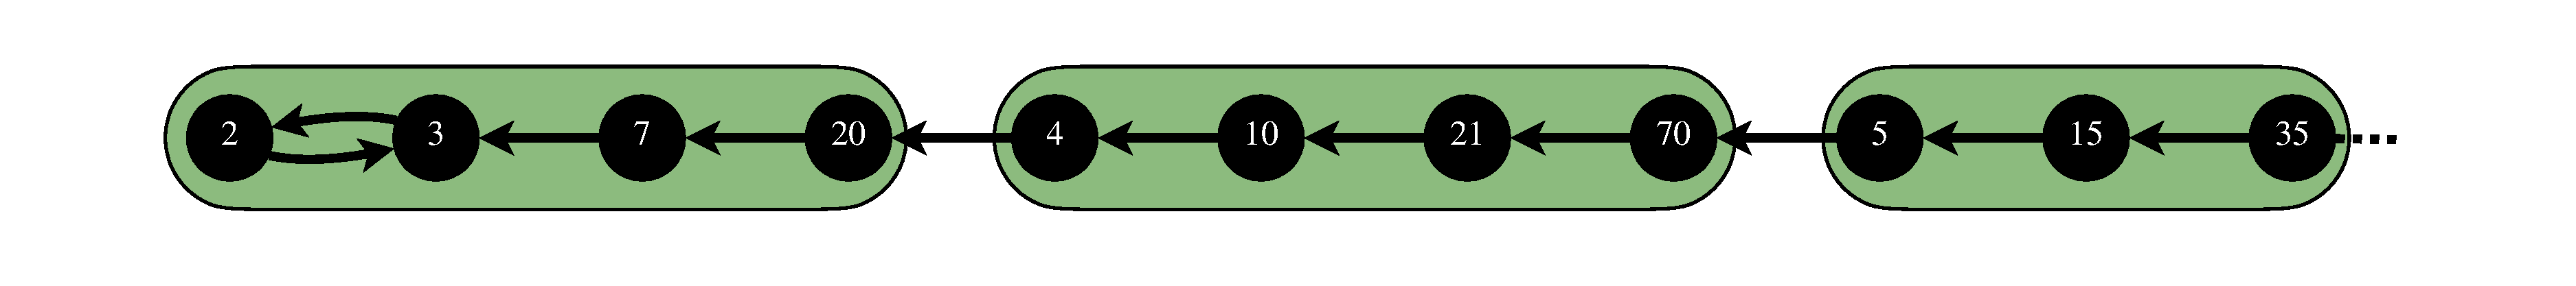
\includegraphics[width=0.9\textwidth]{figures/pathSubchains.pdf}
    \caption{An example describing the partition of a chain into subchains based on cluster sizes.}
    \label{fig:path-subchains}
\end{figure}

We now prove certain key properties about subchains. Let $u_0,u_1,u_2$ denote three contiguous clusters in a chain such that $u_0$ is the last cluster in its subchain, and $u_1$ is the first cluster of its subchain. $u_2$ may or may not belong to the same subchain as $u_1$.

\begin{lemma}\label{lem:path_A}
    If cluster $u_1$ first merges with the cluster (containing) $u_0$, then the weight of the edge $(u_1,u_2)$ reduces to at most $2/3$ times its previous weight.
\end{lemma}
\begin{proof}
    Let $x = w(e)/(S(u_1)S(u_2))$ denote the weight of edge $e=(u_1,u_2)$. If cluster $u_1$ merges with a cluster in its preceding subchain, the merged cluster will be of size at least $S(u_0)+S(u_1)$. Let $x'$ denote the new weight of edge $e$ after this merge. Then,
    \begin{align*}
        x' \le \frac{w(e)}{(S(u_0)+S(u_1))S(u_2)} \implies \frac{1}{x'} &\ge \frac{1}{x} + \frac{S(u_0)S(u_2)}{w(e)}\\
        \implies \frac{1}{x'} &\ge \frac{1}{x} + \frac{S(u_1)S(u_2)}{2w(e)}, & \text{since $S(u_0) \ge S(u_1)/2$}\\
        \implies \frac{1}{x'} &\ge \frac{3}{2x},
    \end{align*}
    Therefore, $x' \le 2x/3$.
\end{proof}

\begin{lemma}\label{lem:path_B}
    If cluster $u_1$ first merges with the cluster (containing) $u_2$, then the weight of the edge $(u_0,u_1)$ reduces to at most $1/3$ times its previous weight.
\end{lemma}
The proof follows by a similar argument as in \Cref{lem:path_A}. By \Cref{lem:path_A,lem:path_B}, each subchain falls into one of the following categories:
\begin{enumerate}[label=(\Alph*)]
    \item The first cluster of the subchain merges with a cluster in the preceding subchain (if exists).
    \item The first cluster of the subchain doesn't merge with a cluster from the preceding subchain.
\end{enumerate}
In either case, one of the edges incident on the first cluster of the subchain moves to a later bucket after it merges, disconnecting the two subchains in the induced graph. Thus, if a subchain falls into category (A), we can move its first cluster to the preceding subchain; if it falls into category (B), we make no changes. By this process, we obtained the modified subchains $C_1',C_2',\ldots,C_K'$, and by the above argument we can run average linkage HAC independently on them. Note that we do not run HAC to completion at these subchains, rather until we have edges with weight within the threshold defined by its bucket. 

Note that the first subchain of a chain will always fall into category (B) since it contains a reciprocal pair which is guaranteed to merge.
Running HAC on this subchain (starting with merging the reciprocal pair) determines whether the next subchain falls into the merge category (A) or (B), which in turn determines the merge category for the following subchain, and so on. 
We now show that we can propagate this merge behavior across subchains with the help of a simple prefix-sum routine in $\poly(\log n)$ depth.

\begin{lemma}\label{lem:path_prefix_sum}
    Given a chain of size $N$ partitioned into subchains $C_1,C_2,\ldots,C_K$, we can determine the merge category ((A) or (B)) for each subchain in $\tilde{O}(N)$ work and $\poly(\log n)$ depth.
\end{lemma}
\begin{proof}
    For subchain $C_j$, let $f(j,A)$ denote the resulting merge category of $C_{j+1}$ if $C_j$ belongs to category (A). Define $f(j,B)$ similarly. Firstly, recall that the category of $C_1$ is determined (it is always category (B)). 
    If $f(j,A) = f(j,B)$, for some $j$, this implies that the category of $C_{j+1}$ is determined regardless of the category of $C_j$. Thus, we can split the chain at subchain $C_{j+1}$ and deal with the two chains obtained, independently. We now assume that $f(j,A)\ne f(j,B)$ for all $j$.

    We create an array $A$ of size $K$ such that,
    \begin{align*}
        A[j] = \begin{cases}
            0 & \text{if $j=1$ and $f(1,B)=A$},\\
            1 & \text{if $j=1$ and $f(1,B)=B$},\\
            0 & \text{if $j>1$ and $f(j,A)=A$},\\
            1 & \text{if $j>1$ and $f(j,A)=B$}.
        \end{cases} 
    \end{align*}
    Let $B= \mathsf{prefix\text{-}sum}(A,\mathtt{XOR},0)$, i.e., $B[1]=0$ and $B[i]=A_1\oplus A_2 \oplus\ldots A_{i-1}$.
    In other words, we compute the prefix sum of the array $A$ with respect to the $\mathtt{XOR}$ function, using $0$ as the left identity element.
    % \lnote{What is $\bot$ here?}
%    \hnote{Shall we define this terminology? Wouldn't prefix ``sum'' be more widely understood?}
    Then, we claim that the merge category of subchain $C_j$ is (A) if $B[j]=0$, otherwise it is (B).

    To see this, consider subchains such that $f(j,A)=A$. These subchains propagate the same category (as them) to the next subchain, which can be viewed as an $\mathtt{XOR}$ operation with a $0$. Similarly, subchains that have $f(j,A)=B$ propagate the opposite category (as them) to the next subchain, which can be viewed as an $\mathtt{XOR}$ with $1$. $A[1]$ denotes the category of subchain $C_2$ that is determined by $C_1$. Thus, computing the $\mathsf{prefix\text{-}sum}$ correctly computes the categories for each subchain.

    The values of $f(j,A)$ (and $f(j,B)$) can be computed by simply simulating average linkage HAC sequentially at each subchain, assuming the category (A) (and (B)) at that subchain. 
    Since the subchain sizes are at most $\log n$, the work incurred to solve HAC on a subchain of size $r$ will be $O(r\log\log n)$.
    
    To see this, consider running Algorithm~\ref{alg:heapbased} on the chain, which we claim runs in $O(N\log\log n)$ work (and depth).
    This is because the heap-based algorithm for HAC (described in more detail in Section~\ref{sec:workupperbound}) on a path containing $r \leq \log n$ elements operates over a heap containing at most $\log n$ elements, and thus each of the at most $r$ merge operations require $O(\log \log n)$ time and only require updating the two neighboring edges incident to the merged edge.
    Since the algorithm used on each subchain is sequential, the depth at each subchain will also be $O(r\log\log n) \in O(\log n\log\log n)$. 
    The $\mathsf{prefix\text{-}sum}$ operation runs in $O(K)$ work and $O(\log K)$ depth. 
    
    Thus, the overall work for a chain containing $N$ elements will be $O(N\log\log n)$ and depth will be $O(\log n\log\log n)$.
\end{proof}

Since the edges are processed in non-increasing order of weight (due to bucketing), and \Cref{lem:path_A,lem:path_B,lem:path_prefix_sum} correctly computes the subchains and proves the correctness of processing these subchains independently, the overall correctness of the algorithm follows directly.

\paragraph{Work and Depth Bounds}
We will now argue the work and depth bounds of the overall algorithm.
Observe that, since the minimum possible weight is at least $W_{\min}/n^2$, the total number of phases will be $T \in O(\log \mathcal{A} + \log n) \in O(\log n)$. 
In each phase, we can compute the nearest neighbor chains in $O(n)$ work and $O(\log n)$ depth; the subchains can also be computed with similar work-depth bounds. By \Cref{lem:path_prefix_sum}, the total work incurred in finding the merge categories for each subchain and running average linkage HAC on these subchains, across all chains, in the worst case will be $O(n\log\log n)$ work and $O(\log n\log\log n)$ depth. Thus, the overall work of the algorithm is $O(n\log n\log\log n)$ and depth is $O(\log^2n\log\log n)$. 

Thus, we have the following theorem about the work and depth of the algorithm:
\mainUpperPar*

\paragraph{Resolving assumptions about chain structure}
\begin{figure}[ht]
    \centering
    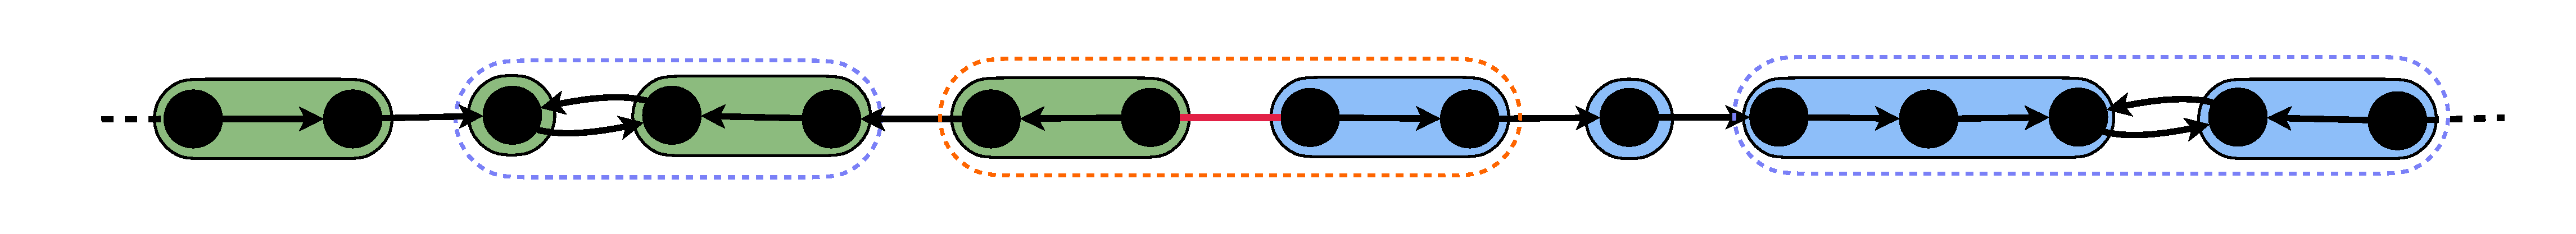
\includegraphics[width=\textwidth]{figures/pathGeneralChains.pdf}
    \caption{An example illustrating the general (possible) structure of the nearest neighbor chains computed in each phase of \Cref{alg:paths}. The red edge here is an example of an edge that is not present in any chain. The dotted lines represents the various subchain merges to address the assumptions made about the nearest neighbor chain structure in \Cref{alg:paths}.}
    \label{fig:path-general-chains}
\end{figure}
We will now address the assumptions made about the structure of chains in the algorithm. When the nearest neighbor chains are computed, the structure of the chains can be represented as 
$$(c'_{N'}\ldots, c_3',c_2', c_1',c_1,c_2,c_3,\ldots,c_{N}),$$
where $(c_1',c_1)$ is the reciprocal pair, $c'_{i-1}$ is the nearest neighbor of $c'_i$, and $c_{i-1}$ is the nearest neighbor of $c_i$. We can extend the idea of partitioning these chains into subchains as follows: partition the chains $(c_1,c_2, \ldots, c_N)$ and $(c'_1,c'_2,\ldots,c'_{N'})$, independently, into subchains using the same criterion as before. Now, merge the subchains containing $c_1$ and $c'_1$ resulting in a subchain of length at most $2\log n$ (see \Cref{fig:path-general-chains}). Then, independently propagate the merge behavior across these two sets of subchains, with the subchain containing $(c_1,c'_1)$ as the first subchain. 

Finally, when we compute the nearest neighbor chains, it is possible for some edges in the bucket to not be present in any chain. However, these edges can occur only between the last vertices of two chains (see \Cref{fig:path-general-chains}). Thus, after finding the merge categories for the subchains containing these vertices (in their respective chains), we can merge these two subchains along with the edge (whose size will be at most $4\log n$ in the worst case). It is not hard to extend the correctness and running time arguments when these modifications are incorporated.

\paragraph{Height of the dendrogram is \texorpdfstring{\boldmath$O(\log^2n)$}{O(log^2(n))}}
An interesting consequence of our algorithm is a constructive proof that the height of the dendrogram obtained when we run average linkage HAC on paths with polynomial aspect ratio is $O(\log^2n)$.



\begin{restatable}{theorem}{pathheight}\label{thm:pathheight}
    Average linkage HAC on path graphs with $\poly(n)$ aspect-ratio returns a dendrogram with height at most $O(\log^2n)$.
\end{restatable}

\begin{proof}
    Starting with phase 1, the algorithm runs average linkage HAC (partially) on independent $O(\log n)$-sized contiguous portions (i.e., subchains) of the path. Thus, each subchain will correspond to independent parts in the output dendrogram. Since there are $O(\log n)$ phases and the max-height generated in each phase is at most $O(\log n)$, we get an overall bound of $O(\log^2n)$ for the height in the worst case.
\end{proof}


% the algorithm partitions the edges into \emph{buckets} such that edges in each bucket have equal similarity, up to constant factors. Since the minimum possible similarity for an edge is at least $W_{\min}/n^2$, the number of buckets ($T$) will be in $O(\log \mathcal{A} + \log n) \in O(\log n)$ (due to bounded aspect ratio). Then, the algorithm runs in phases where in the $t$-th phase it computes the nearest neighbor chains in the induced graph $G[B_t]$. processes only edges from $B_t$, and computes the nearest neighbor chains


% \begin{itemize}
%     \item Partition the edges into buckets $B_1, B_2, \ldots, B_t$, where $B_i$ maintains edges with similarity in the range $((2/3)^{i}w_{\max}, (2/3)^{i-1}w_{\max}]$. Observe that, since the minimum possible similarity is at least $w_{\min}/n^2$, $t \in O(\log \mathcal{A} + \log n) \in O(\log n)$.
%     \item Run the following algorithm in $t$ phases. 
%     In the $i^{th}$ phase, the algorithm only considers edges in $B_i$ and pushes edges to later buckets as soon as their similarity drops below the threshold of $B_i$.
%     \begin{enumerate}
%         \item Compute the nearest neighbor chains. 
%         \hnote{We can add a pseudocode and some illustration to explain the algorithm here. We could also add an informal explanation first. Why NN chains are relevant and what subchains denote are not clear to the lay reader. The enumeration here is really not an algorithm, rather the description of the algorithm intertwined with notes about the proof. May be a good idea to decouple. I would avoid the bullet point style presentation in this section.}
%         We make the following two assumptions about these chains; we later show how to remove these assumptions.
%         \begin{itemize}
%           \item Each chain can be represented as $(v_1,v_2, v_3, \ldots, v_\ell)$ such that $v_{i-1}$ is the nearest neighbor of cluster $v_i$, and $(v_1,v_2)$ is the \emph{reciprocal pair}. Thus, the similarities are in non-increasing order from left to right.
%           \item Every edge in $B_i$ is present in some chain.
%         \end{itemize}
%         By these assumptions, each chain will be a separate connected component in the graph induced on $B_i$. Thus, we process each chain independently.
%         \item Fix some chain. Partition it further into a set of \emph{subchains}, where a subchain $(u_1, u_2, u_3, \ldots, u_s)$ is a \emph{contiguous} set of clusters such that $S(u_{i}) \ge 2S(u_{i-1})$. Observe that the size of a subchain cannot exceed $\log n$. Thus, we can afford to sequentially process each subchain. Additionally, we always include $v_1$ in the subchain containing $v_2$.
%         \item For a subchain $(u_1, u_2, u_3, \ldots, u_s)$, let $u_0$ denote the last vertex in the subchain preceding it in its chain (if exists). We have two ``merge categories'' here:
%         \begin{enumerate}[label = (\Alph*)]
%             \item $u_1$ first merges with some cluster in the preceding subchain: In this case, we will show that the similarity of edge $(u_1,u_2)$ reduces to at most $2/3$ times its previous similarity after this merge (see \Cref{lem:path_A}), thus pushing it to a later bucket.
%             \item $u_1$ first merges within its subchain: In this case, we will show that the similarity of edge $(u_0,u_1)$ reduces to at most $1/3$ times its previous similarity after this merge (see \Cref{lem:path_B}), thus pushing it to a later bucket.
%         \end{enumerate}
%         Thus, once we figure out the merge category for each subchain, we can run average-linkage HAC independently. Note that we do not run HAC to completion at these subchains, rather until we have edges with similarity within the threshold defined by $B_i$.
%         \item Note that the first subchain of a chain would always fall into category (B). Running HAC on this subchain (starting with merging the reciprocal pair) determines whether the next subchain falls into the merge category (A) or (B), which in turn determines the merge category for the following subchain, and so on. We can propagate this merge behavior across subchains with the help of a simple prefix-sum routine in $\tilde{O}(1)$ depth (see \Cref{lem:path_prefix_sum}).
%         \item Once the appropriate merge category ((A) or (B)) is determined at each subchain, run average-linkage HAC at each subchain, in parallel, until either all edges are merged or pushed to a later bucket.
%     \end{enumerate}
% \end{itemize}


% TODO:
% - If figured out, discuss how to extend this algorithm to trees, assuming oracle access to a CC-complete problem.